\documentclass[12pt,a4paper]{report}
\usepackage{geometry}
\geometry{
	a4paper,
	total={170mm,257mm},
	left=20mm,
	top=20mm,
}\usepackage{graphicx}
\usepackage{tcolorbox}
\usepackage{mathtools}
\usepackage{tabu}
\tcbuselibrary{breakable}
\usepackage{listings}
\usepackage{xepersian}
\settextfont[Scale=1]{BNazanin}
\setlatintextfont[Scale=1]{Calibri}
\renewcommand{\baselinestretch}{1.5} 



\begin{document}
	\begin{titlepage}
		\centering
		
\includegraphics[width=0.45\textwidth]{Figures/logo}\par\vspace{1cm}
		{\scshape\LARGE  دانشکده مهندسی برق و کامپیوتر دانشگاه تهران \par}
		\vspace{1cm}
		{\scshape\Large  گزارش فصل 1: \lr{Single Server Queuing Model}\par}
		\vspace{1.5cm}
		{\huge\bfseries امیرحسین مرادیان\par}
		\vspace{0.5cm}
		{\Large\itshape 810100467\par}
		\vfill
		\huge {استاد درس:}
		\par
		دکتر خونساری
		
		\vfill
		
		% Bottom of the page
		{\large \today\par}
	\end{titlepage}
	
	\pagebreak
	
	\section*{مقدمه}
	
	سیستم به این صورت عمل می کند که مشتری وارد می شود و سرور را بیکار پیدا می کند و بلافاصله از سیستم سرویس می گیرد. لازم به ذکر است که زمان های سرویس دهی از مشتریان متوالی نیز متغیر های تصادفی$ IID$ هستند که مستقل از زمان های بین ورود می باشد. حال اگر یک مشتری وارد شود و سرور را مشغول بیابد، به انتهای صف می رود. زمانی که سرویس دهی به یک مشتری تکمیل می شود، سرور صف را چک کرده و در صورتی که مشتری در صف وجود داشته باشد، آن را به روش $ FIFO $ انتخاب می کند.

	شبیه سازی در حالت خالی صف و بیکار سرور آغاز می شود. در زمان صفر، ما شروع به انتظار برای ورود اولین مشتری خواهیم کرد که پس از اولین زمان بین ورود یا همان $A_1$، به جای زمان 0 (که یک فرض مدل سازی احتمالاً معتبر، اما متفاوت است) رخ می دهد. ما میخواهیم این سیستم را تا زمانی شبیه سازی کنیم که تعداد مشخصی مشتری (که آن را$ n $می نامیم) تاخیر های خود را در صف تکمیل کنند. به عبارت دیگر، زمانی که$ n$ مین مشتری وارد سرویس شود، شبیه سازی متوقف می شود ، زمان پایان شبیه سازی نیز یک متغیر تصادفی است.
	
	برای سنجش عملکرد این سیستم سه کمیت را برآورد خواهیم کرد. اولین کمیت، میانگین تاخیر مورد انتظار در صف برای$ n $مشتری خواهد بود .در این راستا، در یک اجرای معین از شبیه سازی، میانگین تاخیر واقعی مشاهده شده از$ n $مشتری به مشاهدات متغیر تصادفی بین ورود و زمان سرویس دهی بستگی دارد. این در حالی است که در اجرای دیگری از شبیه سازی، احتمالاً زمان های مختلفی برای زمان ورود سرویس دهی را شاهد خواهیم بود که این دلیلی بر درستی در نظر گرفتن میانگین$ n $به عنوان یک متغیر تصادفی است. چیزی که ما در این شبیه سازی به دنبال آن هستیم، برآورد میانگین تاخیر مورد انتظار  مشتری است که آن را با $d(n)$ نمایش می دهیم و به صورت زیر آن را تعریف خواهیم کرد :
	\begin{equation}
		\hat{d}(n) = \frac{\Sigma^n_{i = 1} D_i}{n}
	\end{equation}
	یکی دیگر از این معیارها برای ارزیابی مدل میانگین مورد انتظار تعداد مشتریان در صف است (مشتریانی که به آنها سرویس دهی نمی شود)، که این کمیت را با $q(n)$ نمایش می دهیم. این یک نوع متوسط متفاوت از میانگین تاخیر در صف است، چرا که به جای مشتریان (گسسته بودن) زمان (پیوسته) گرفته می شود. بنابراین ما باید تعریف کنیم که منظور از این تعداد میانگین زمانی مشتریان در صف چیست. برای انجام این کار $Q(t)$ را تعداد مشتریان در صف در زمان$ t$ تعریف کرده و $T(n)$ را زمان مورد نیاز برای مشاهده$ n$ تاخیر در صف در نظر میگیریم. به این صورت، برای هر زمان $t$ بین 0 و $T(t)$،$ًًQ(n)$ یک عدد صحیح غیر منفی است. همچنین اگر $p_i$ را نسبت مورد انتظار که بین 0 و 1 خواهد بود، از زمانی که $Q(t)$ برابر با$ i $است بگذاریم، به رابطه زیر خواهیم رسید :
	
	\begin{equation}
		\hat{q}(n) = \frac{\int^{T(n)}_0 Q(t) dt}{T(n)}
	\end{equation}

	سومین معیار ارزیابی عملکرد برای این سیستم، میزان شلوغی سرور است. استفاده مورد انتظار از سرور، نسبت زمان مورد انتظار در طول شبیه سازی (از زمان 0 تا زمان T(n) ) است که سرور مشغول است ، و بنابراین عددی بین 0 و 1 است و آن را با $u(n)$ نشان می دهیم. پس از یک شبیه‌سازی، تخمین ما از $u(n)$ برابر است با نسبت مشاهده‌شده در طول شبیه‌سازی که سرور مشغول است. اکنون $\hat{u}(n)$ را می‌توان مستقیماً از شبیه‌سازی با ذکر زمان‌هایی که در آن سرور وضعیت تغییر می‌کند (تغییر از بی‌کار به مشغول یا برعکس) و سپس انجام تفریق و تقسیم مناسب محاسبه کرد. با این حال، با تعریف "عملکرد مشغول" ساده تر است که به این کمیت به عنوان یک میانگین زمان پیوسته، مشابه طول متوسط صف نگاه کنیم.
	\begin{align*}
		B(t) = 
		\begin{cases}
			1 & $ \lr{if the server is busy at time t }$ \\
			0 & $ \lr{if the server is idle at time t} $
		\end{cases}
	\end{align*}
	و بنابراین $\hat{u}(n)$ را می توان به عنوان نسبت زمانی بیان کرد که $B(t)$ برابر با 1 است. با این حال با توجه به اینکه ارتفاع تابع $B(t)$ همواره بین 0 و 1 است و معیار مورد نظر ما را می توان به عنوان مساحت زیر تابع $B(t)$ در طول شبیه سازی در نظر گرفت، خواهیم داشت:
	\begin{equation}
		\hat{u}(n) = \frac{\int^{T(n)}_0 B(t) dt}{T(n)}
	\end{equation}

	\pagebreak
	
	\section*{\lr{MATLAB Code}}
	
	
	کد های متلب زده شده مرتبط با پروژه را در زیر میتوانید مشاهده کنید:
	در ابتدا میتوانید تایع 
	\lr{arrive}
	را که نشان دهنده رسیدن به سرور هست را مشاهده کنید:\\
	
	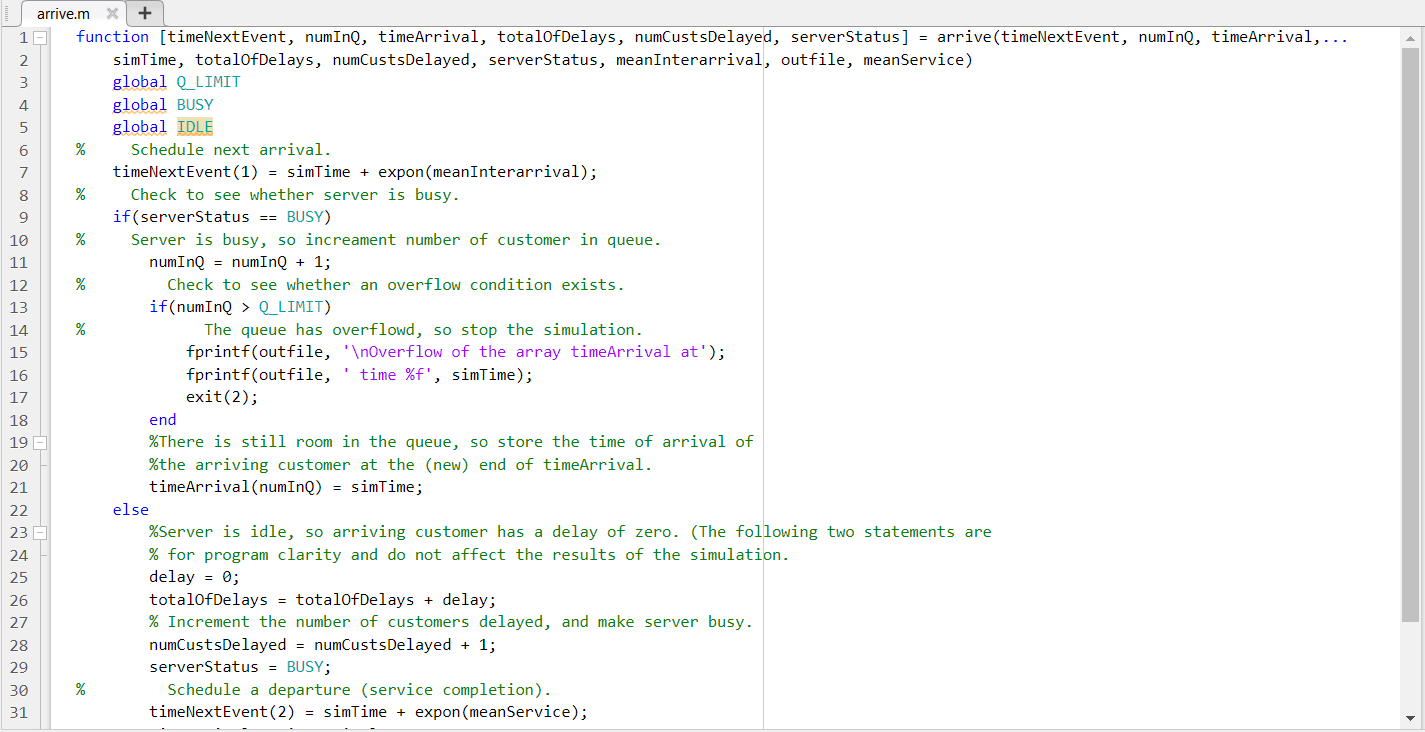
\includegraphics[scale=0.6]{Figures/A1}
	
	در شکل زیر ادامه کد را خواهید دید:
	
	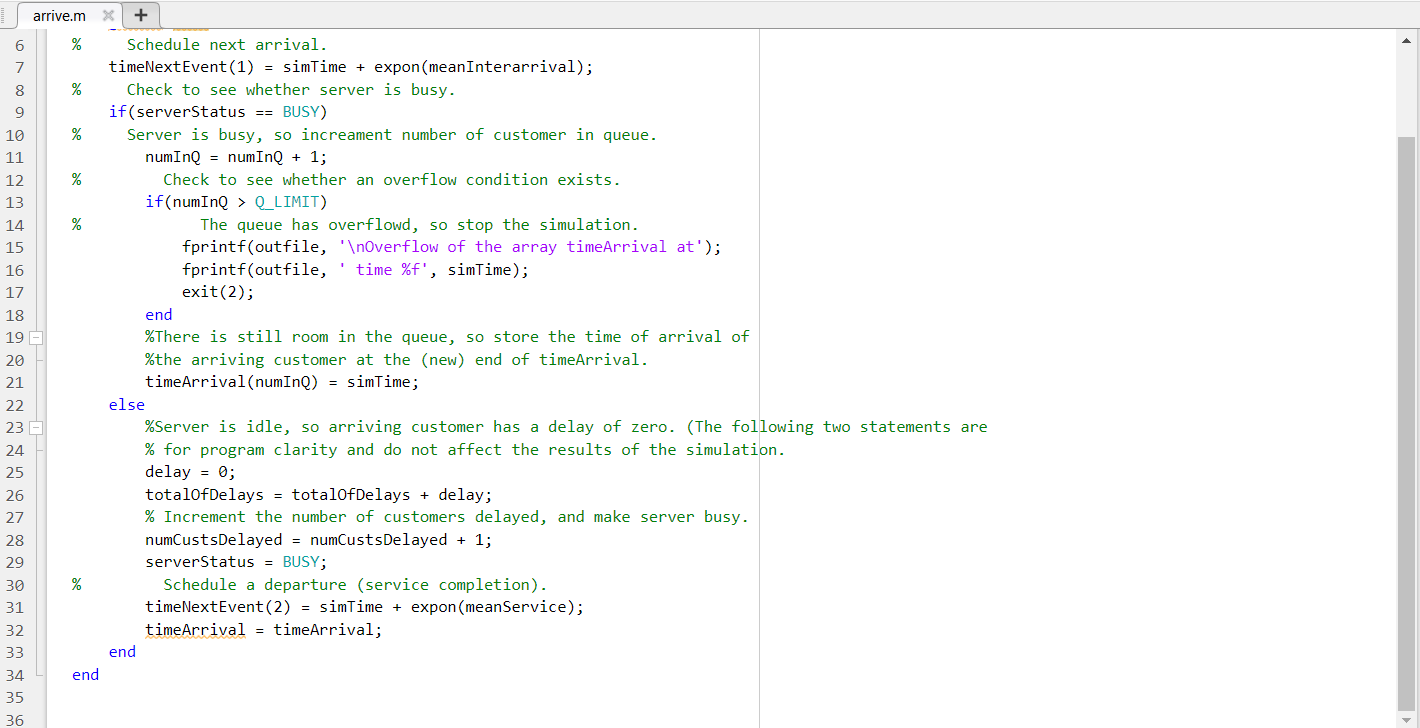
\includegraphics[scale=0.6]{Figures/A2}
	
	\pagebreak
	
	در کد زیر تابع جداشدن را از سرور میتوانید مشاهده کنید:\\
	
	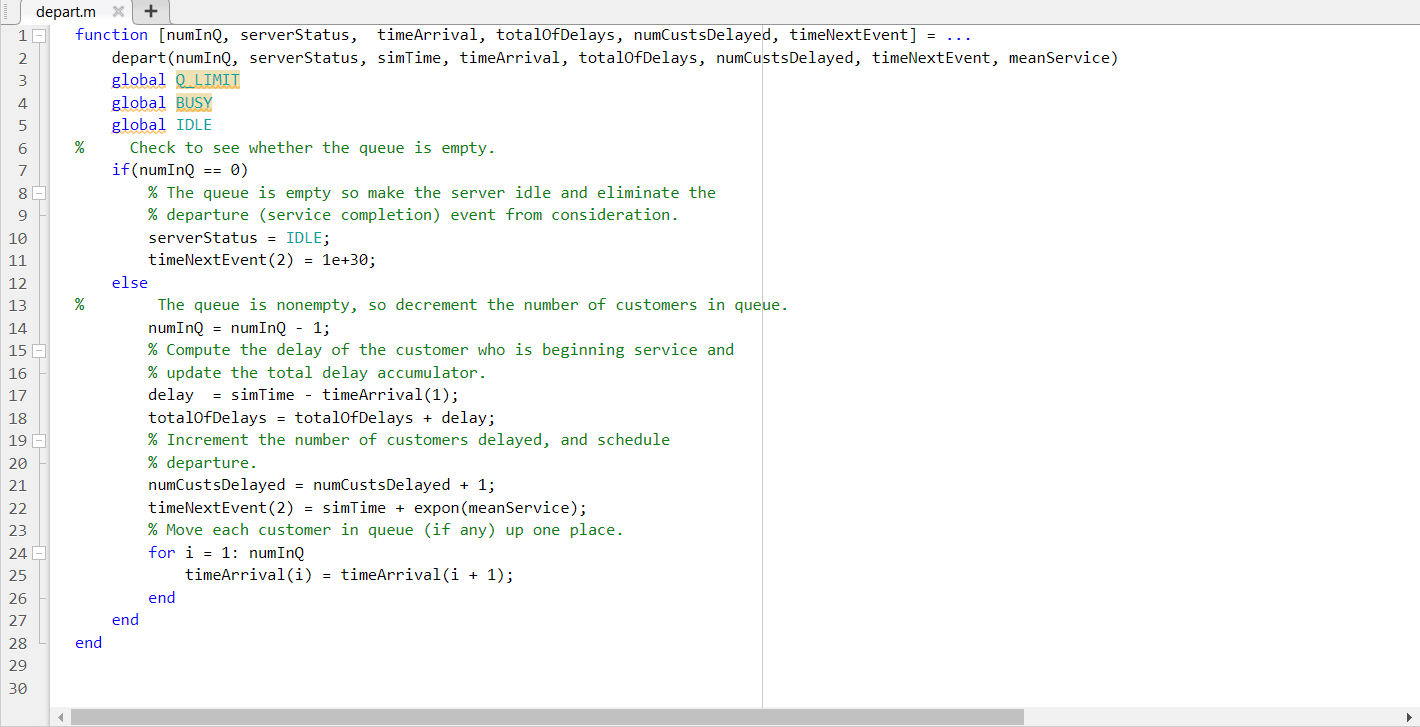
\includegraphics[scale=0.6]{Figures/D}
	
	در زیر میتوانید تابع 
	\lr{exponential}
	را مشاهده کنید\\
	
	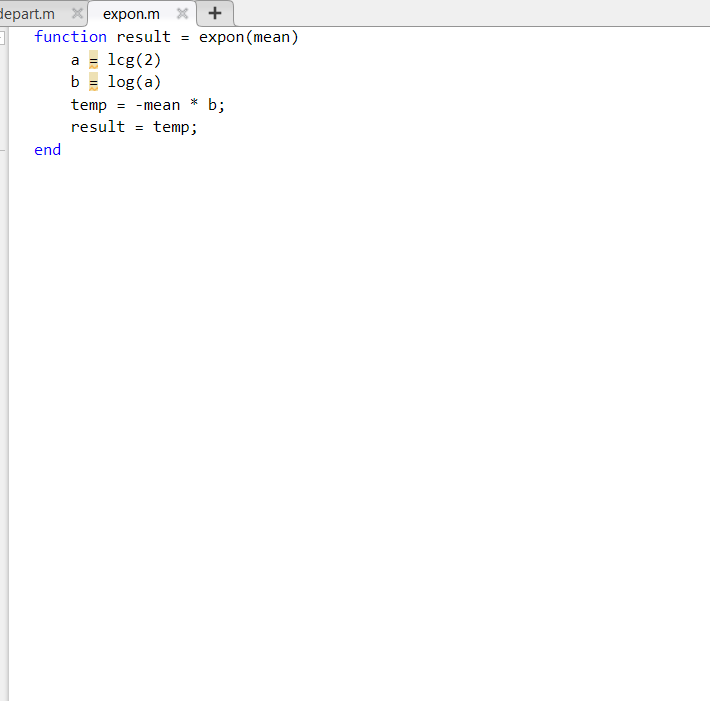
\includegraphics[scale=0.6]{Figures/E}
	
	\pagebreak
	
	در این بخش  
	\lr{Initialize}
	را مشاهده میکنید:\\
	
	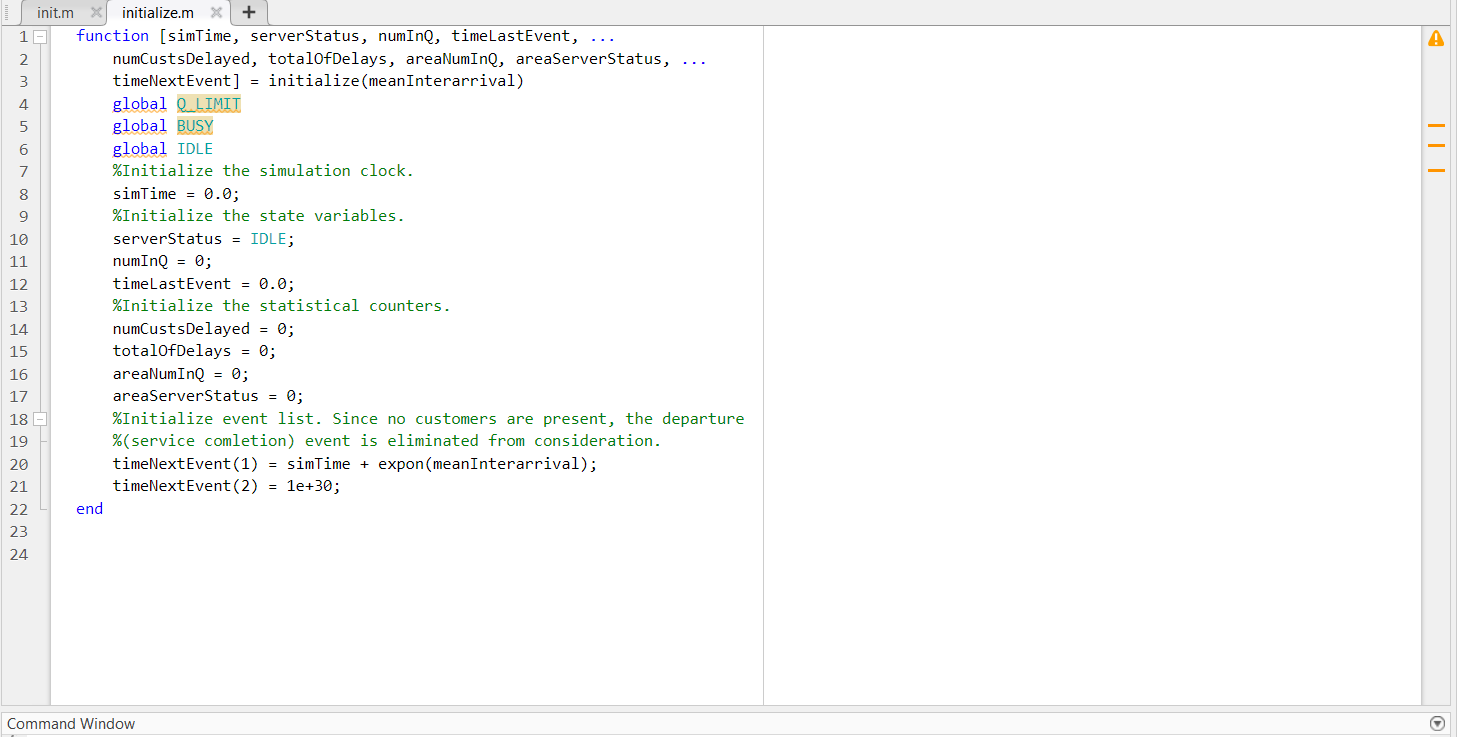
\includegraphics[scale=0.6]{Figures/I}
	
	
	اکنون کد مربوط به بخش
	\lr{lcg}
	را میتوانید مشاهده کنید:\\
	
	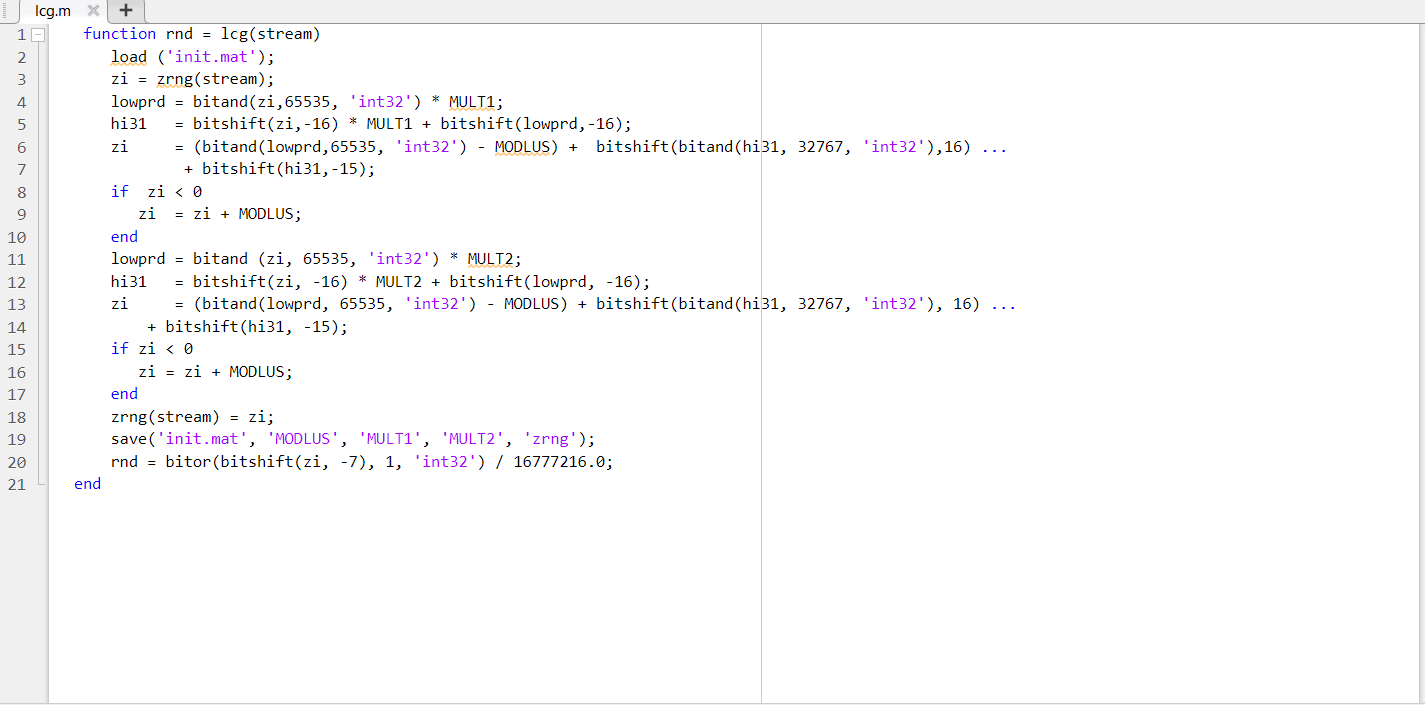
\includegraphics[scale=0.6]{Figures/L}
	\pagebreak
	در ادامه میتوانید بخش 
	\lr{Report}
	را مشاهده کنید:
	
	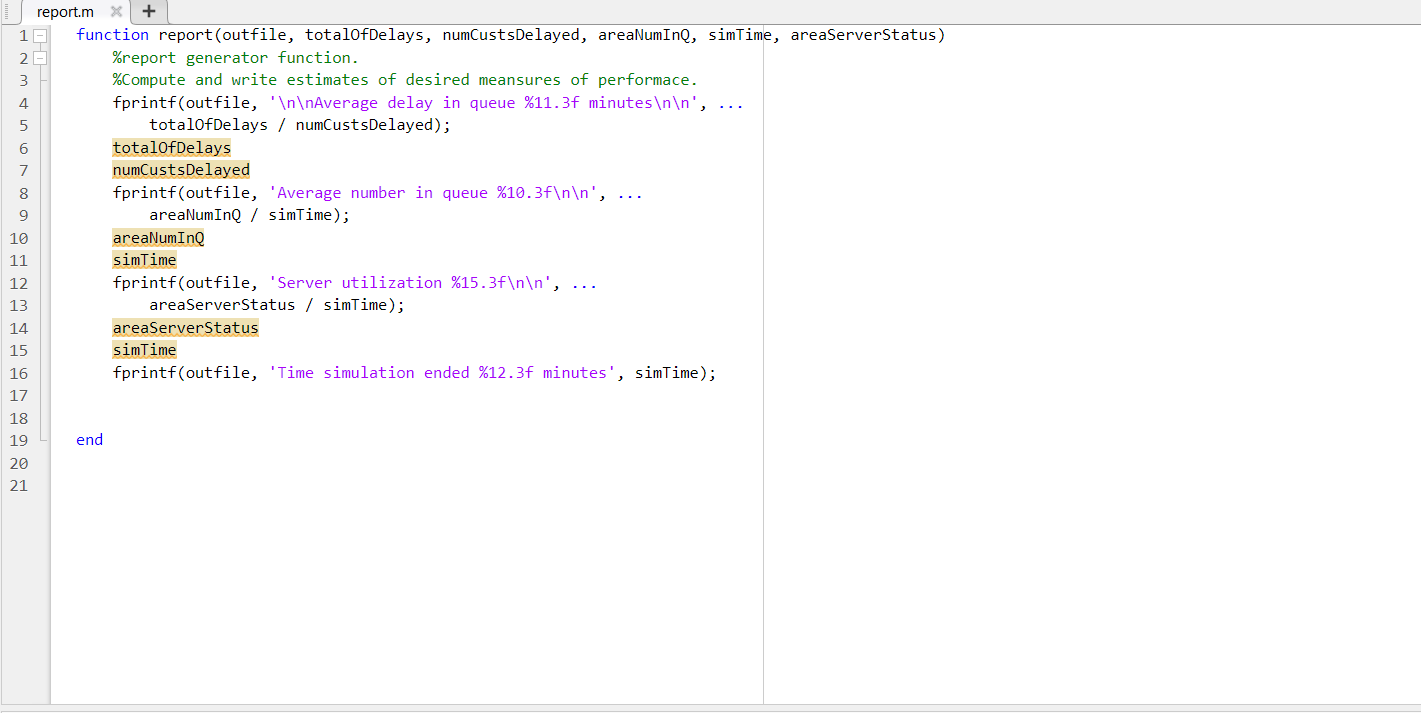
\includegraphics[scale=0.6]{Figures/R}
	
	و همچنین تابع 
	\lr{Timing}
	را میبینید:
	
	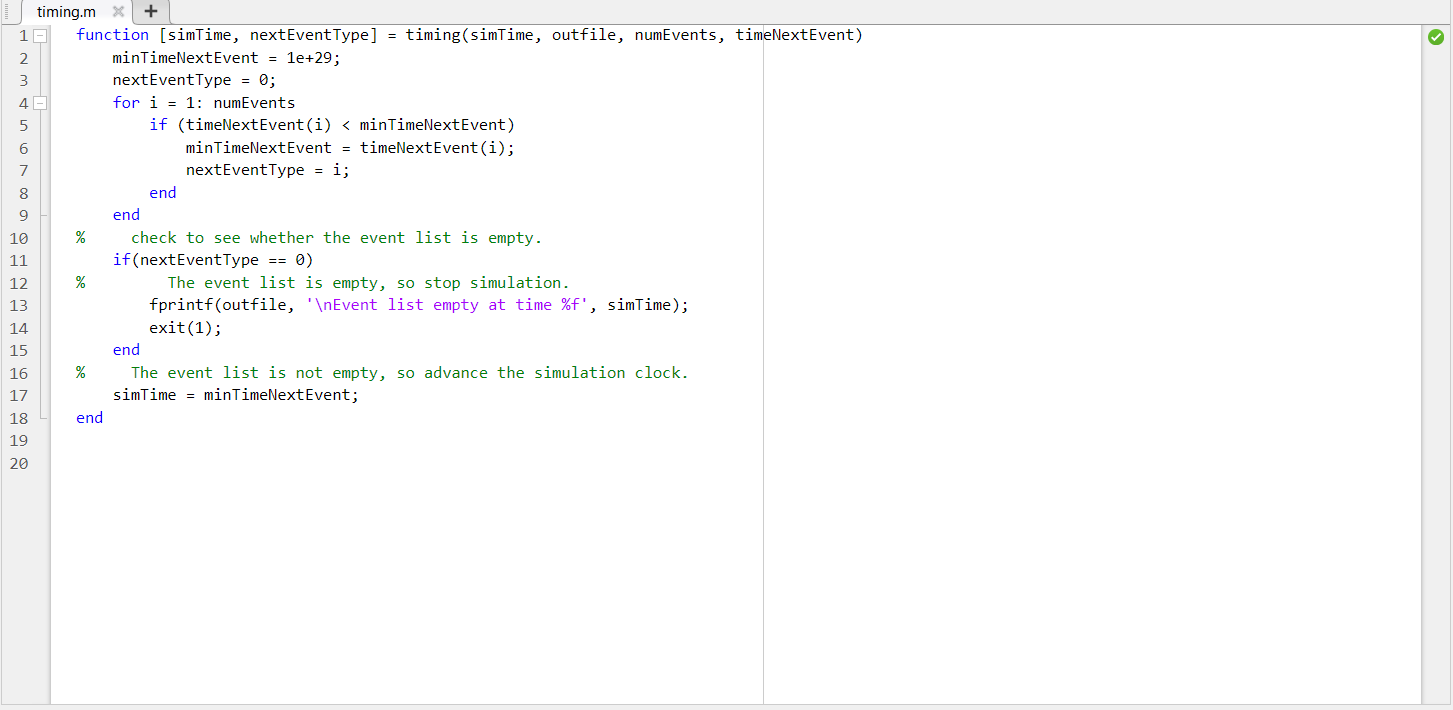
\includegraphics[scale=0.6]{Figures/T}
	
	\pagebreak
	
	و در نهایت آخرین تابع تحت عنوان
	\lr{UpdateTimeArrival}
	که زمان رسیدن به سرور را به روز رسانی میکند در زیر آمده است:
	\\
	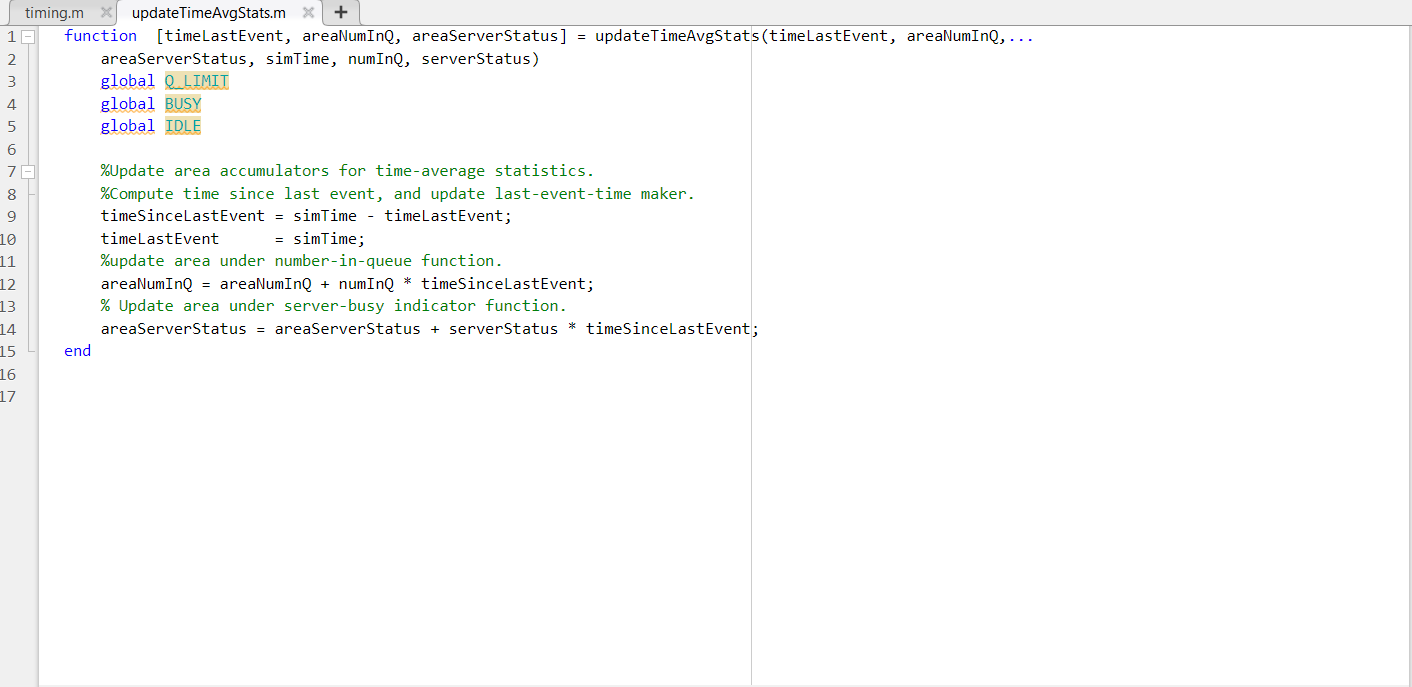
\includegraphics[scale=0.6]{Figures/U}
	
	
	
	تمامی کد های متلب در بالا به همراه توضیحات لازم آورده شده اند. میتوانید مشاهده کنید. 
	
	
	
\end{document}